\chapter{Deployment of Cognitive Relay}
\label{chap:Deploy}
Using software defined radio.
\section{Interweave System}
Hardware demonstration \cite{Kaushik_ISWCS} of \ac{CR} that
\begin{itemize}
\item detects spectrum holes or temporal opportunities in \ac{PU} system 
\item illustrates cognitive sensing ,i.e, it estimates the spectral occupancy for the multi-band \ac{PU} system
\end{itemize}
\section{Underlay System}
\ac{CR} operating as underlay system \cite{Kaushik_CROWNCOM}
\begin{itemize}
\item deploys propagation models to capture movements of \ac{PR} and \ac{ID}
\item implements sharing constraints to access the \ac{PU} channel 
\end{itemize}

%\index{Family Radio Service}
%\subsection{Overview of the standard}
%\ac{FRS} is a communication system that is used for speech transmission within a range of less than one mile. Therefore, the transmitters have a maximum output power of \SI{500}{mW}. The signal is modulated with an \ac{FM}\index{Frequency modulation} scheme, where the envelope of the complex baseband signal $s_\text{tx}(t)$ can be described as follows:
%\begin{equation}
%s_\text{tx}(t) = \exp \left(j 2 \pi  f_\Delta \int_0^t v(t') dt' \right),
%\label{eq:fm}
%\end{equation} 
%
%where $v(t)$ is the audio signal that should be transmitted and $f_\Delta$ describes the frequency deviation. FRS is a narrowband FM system and is intended for channels with \SI{12.5}{kHz} bandwidth. Therefore, $f_\Delta$ is set to \SI{2.5}{kHz} while the maximum frequency of the audio signal $v(t)$ should not exceed \SI{3.5}{kHz}. The \ac{FCC} specified 14 channels between \SI{462.5625}{MHz} and 	\SI{467.7125}{MHz}. This means that the carrier frequency is in the same range as the TETRA waveform and can be achieved with the same RF front ends.
%
%\subsection{Digital signal approximation for the portability}
%In a digital representation, the integral in equation (\ref{eq:fm}) can be replaced by a sum of the values coming from the sound card. These values are scaled with the frequency deviation factor and synthesize the angle for the complex base band signal. The receiver works vice versa. The angle of the incoming in-phase and quadrature component is determined and scaled. The audio signal can be retrieved by subtraction of the previous angle from the current angle. 
%
%
%\subsection{Results}
%Due to the narrow bandwidth of \SI{12.5}{kHz}, a high resampling has to be applied. However, the signal has just to be resampled to a data rate that the sound card supports. In case of the USRP this is \SI{32}{kHz}. Together with the ADC rate of \SI{64}{MHz}, this leads to a decimation rate of 2000 in the FPGA. The audio system on the SFF can be coupled to the FPGA data rate. Therefore, the same rates as for the TETRA waveform was applied leading to a reuse of the decimation, interpolation and downconversion.
%
%Since the transmitter comprises only an integration and the receiver consists only of a differentiator beside the resampling filters, the whole \ac{PIM} can be shifted to the GPP, DSP or even FPGA without any modifications. This shows that if the processing power of the underlying platform is amply dimensioned for the complexity and bandwidth of the waveform, the concerned waveform here can be ported without any knowledge of the underlying hardware.
%
%
%\section{Wireless LAN in the version IEEE 802.11g}
%\index{WLAN}
%\index{IEEE 802.11g}
%
%\subsection{Overview of the standard}
%Since 1980, the \ac{IEEE} releases specifications about Local Area Networks (LANs) in its project 802. In 1997, the first specification of a \ac{WLAN} was published within the working group eleven. This was the beginning of the standard IEEE 802.11, which specifies \ac{MAC} and \ac{PHY} for local radio networks. In the original version, data rates up to \SI{2}{Mbit/s} were reached with spread spectrum techniques in the \SI{2.4}{GHz} \ac{ISM}\index{ISM radio band} radio band. Just about two years later, in 1999, the standard was extended with two annexes. IEEE 802.11a specified an \ac{OFDM} transmission in the \SI{5}{GHz} \ac{ISM} band with data rates up to \SI{54}{Mbit/s} and 802.11b extended the transmission on \SI{2.4}{GHz} to data rates up to \SI{11}{Mbit/s}. The most common extension till the present day is annex g, which was released in 2003 and specified the \ac{OFDM}\index{OFDM} transmission with up to \SI{54}{Mbit/s} in the \SI{2.4}{GHz} range \cite{IEEE802.11}. This is a frequency range that is supported by the Flex2400 daughter board for the USRP and the WiMAX module RF front end for the SFF as described in sections \ref{sec:USRP} and \ref{sec:SFF}.
%
%\subsection{Challenges for the portability of the waveform}
%The major challenge in implementing and porting the 802.11g waveform is its large bandwidth. The symbol duration of one OFDM symbol is specified to \SI{3.2}{\micro s}. This results in a bandwidth of \SI{20}{MHz} with 64 subcarriers. Even if the data converters on both platforms can support this bandwidth, the buses between DSP/GPP and FPGA are not fast enough. By assuming 16 bit in-phase and quadrature components, data rates of \SI{640}{Mbit/s} must be achieved, while the maximum data rate between GPP and FPGA on the USRP is \SI{228}{Mbit/s} and the maximum data rate on the SFF SDR DP is \SI{52}{Mbit/s}. This means that the complete waveform should be implemented on the FPGA. However, both platforms provide not enough logic to achieve this. Due to the fact that no real time implementation is possible with the given platforms, the maximum achievable bandwidths should be evaluated. Therefore, a \ac{PIM} was realized with the channel from section \ref{sec:PIM_TETRA}. To achieve a synchronization in time and frequency, an algorithm from Schmidl and Cox\index{Schmidl and Cox synchronization} \cite{schmidl_cox} was realized that uses training sequences in the beginning of each transmission to find the exact position of an OFDM symbol in the data stream coming from the \acp{ADC}. 
%
%\begin{figure}[htb]
%	\centering
%		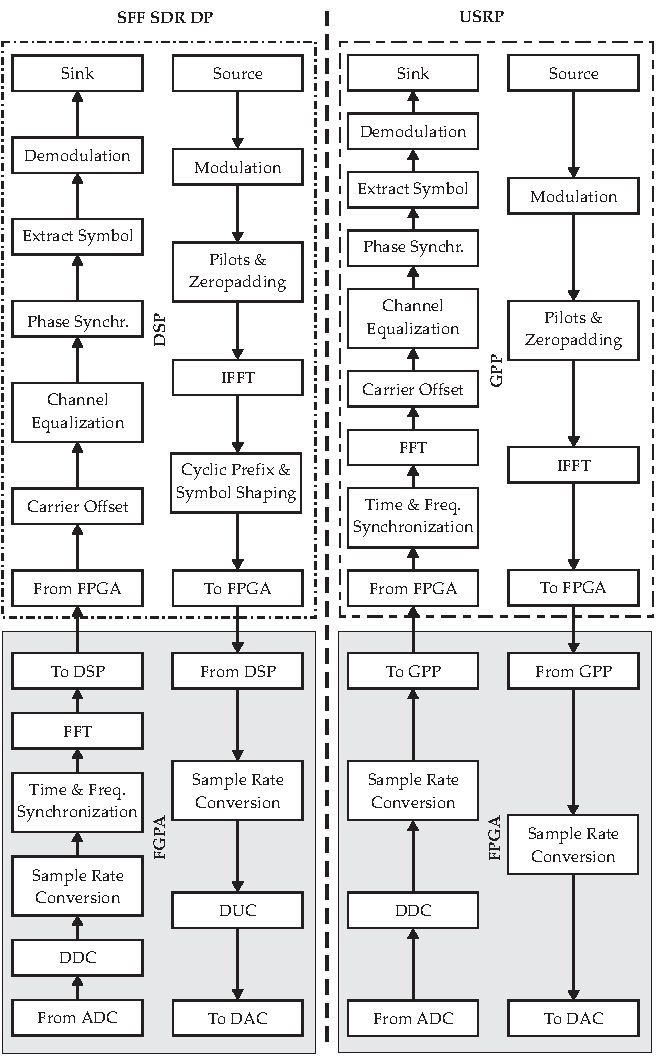
\includegraphics[height=0.9\textheight]{../kapitel05/figures/OFDM_b.pdf}
%	\caption{Separation of the waveform for the processing elements on USRP and SFF SDR}
%	\label{fig:OFDM_b}
%\end{figure}
%
%\subsection{Results}
%To fulfill the real time constraints for 802.11g, the time for one OFDM symbol with the guard interval must not exceed \SI{4}{\micro s}. Measurements on the Intel P8400 showed that the processing time for the transmitter is approximately \SI{2.78}{\micro s}. Without the limitation due to the bus between GPP and FPGA, it is possible to implement the transmit side in software and support the real time constraints of a \SI{20}{MHz} bandwidth. However, due to the fact that the maximum data rate of the bus is at \SI{228}{Mbit/s}, only a bandwidth of \SI{6.4}{MHz} can be achieved. The spectrum of the transmitted signal was recorded with a Rohde \& Schwarz FSQ8 signal analyzer and is shown in figure \ref{fig:spec_ofdm_data}. To detect the 802.11g frame, a training sequence was transmitted where its spectrum is shown in figure \ref{fig:spec_ofdm_sts}. The representation of the spectrum shows the power in a logarithmic scale.
%
%The processing time for the receiver is \SI{58.9}{\micro s}. Therefore, with the used processor, a whole system comprising of transmitter and receiver with a USRP can only be realized with a complex bandwidth of up to \SI{1.3}{MHz}. This is due to the timing and error synchronization as well as the Viterbi decoding. These two processing blocks consume \SI{75}{\%} of the processing time for one OFDM symbol.
%
%When porting the code for the transmitter from the USRP to the SFF SDR a processing time of \SI{600}{\micro s} was measured for one OFDM symbol. As already mentioned in section \ref{sec:bench_dsp}, this is due to the floating point implementation. The data section of the code becomes too large for the internal memory and has to use the slow external SDRAM. The usage of external memory can be circumvented with a fixed point design and the use of optimized libraries as presented in section \ref{sec:overhead}. With these changes the processing time for an OFDM symbol decreases to \SI{18.9}{\micro s}.
%
%The transformation of the \ac{PIM} for the receiver yields similar results. The measurements of the floating point code lead to a processing time of \SI{222}{ms}. Even with a fixed point implementation of the model, the memory size exceeds the internal cache. Therefore, the timing and frequency synchronization must be shifted to the FPGA. The sample based processing on this reconfigurable logic requires a completely new modeling of the synchronization algorithm. Especially the peak detection of the correlation must be redesigned. Nevertheless, the processing time for one OFDM symbol in the receiver could be decreased to \SI{12.4}{ms}. This time could be further reduced with an optimized version of the Viterbi algorithm. Similar to the results on the USRP, this is the processing block that consumes most of the time.
%
%The realization of the \acp{PSM} for the USRP and the SFF SDR are shown in figure \ref{fig:OFDM_b}. The porting process for this waveform is described in more details in \cite{nagel_frequenz} and \cite{pwd}.
%
%
%
%%\begin{figure}
%%\centering
%%\subfigure[Power spectrum of the waveform data\label{fig:spec_ofdm_data}]{\includegraphics[width=0.8\textwidth]{../kapitel05/figures/Freq_FSQ8_Data.pdf}}
%%\hfill
%%\subfigure[Power spectrum of the training sequence\label{fig:spec_ofdm_sts}]{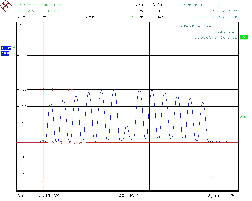
\includegraphics[width=0.8\textwidth]{../kapitel05/figures/Freq_FSQ8_STS.pdf}}
%%\caption{Measured power spectrum in dBm of the OFDM waveform}
%%\end{figure}
%
%%\section{Universal Mobile Telecommunication System}
%%
%%\subsection{Overview}
%%UMTS
%%CDMA
%%DSSS
%%channel versus OVSF
%%cells versus gold codes
%%two channels for synchronization: PSC and SSC
%%
%%\subsection{Challenges}
%%timing synchronization and resampling through polyphase filters
%%slot synchronization  over correlation with the PSC
%%frame synchronization over ssc
%%
%%\subsection{Results}
%%1.1 s
%%no sff implementation
%%similar results as for ofdm
